\documentclass[]{article}
\usepackage{lmodern}
\usepackage{amssymb,amsmath}
\usepackage{ifxetex,ifluatex}
\usepackage{fixltx2e} % provides \textsubscript
\ifnum 0\ifxetex 1\fi\ifluatex 1\fi=0 % if pdftex
  \usepackage[T1]{fontenc}
  \usepackage[utf8]{inputenc}
\else % if luatex or xelatex
  \ifxetex
    \usepackage{mathspec}
  \else
    \usepackage{fontspec}
  \fi
  \defaultfontfeatures{Ligatures=TeX,Scale=MatchLowercase}
\fi
% use upquote if available, for straight quotes in verbatim environments
\IfFileExists{upquote.sty}{\usepackage{upquote}}{}
% use microtype if available
\IfFileExists{microtype.sty}{%
\usepackage{microtype}
\UseMicrotypeSet[protrusion]{basicmath} % disable protrusion for tt fonts
}{}
\usepackage[margin=1in]{geometry}
\usepackage{hyperref}
\hypersetup{unicode=true,
            pdftitle={DATA 606 - Lab 7},
            pdfauthor={Joshua Sturm},
            pdfborder={0 0 0},
            breaklinks=true}
\urlstyle{same}  % don't use monospace font for urls
\usepackage{color}
\usepackage{fancyvrb}
\newcommand{\VerbBar}{|}
\newcommand{\VERB}{\Verb[commandchars=\\\{\}]}
\DefineVerbatimEnvironment{Highlighting}{Verbatim}{commandchars=\\\{\}}
% Add ',fontsize=\small' for more characters per line
\usepackage{framed}
\definecolor{shadecolor}{RGB}{248,248,248}
\newenvironment{Shaded}{\begin{snugshade}}{\end{snugshade}}
\newcommand{\KeywordTok}[1]{\textcolor[rgb]{0.13,0.29,0.53}{\textbf{#1}}}
\newcommand{\DataTypeTok}[1]{\textcolor[rgb]{0.13,0.29,0.53}{#1}}
\newcommand{\DecValTok}[1]{\textcolor[rgb]{0.00,0.00,0.81}{#1}}
\newcommand{\BaseNTok}[1]{\textcolor[rgb]{0.00,0.00,0.81}{#1}}
\newcommand{\FloatTok}[1]{\textcolor[rgb]{0.00,0.00,0.81}{#1}}
\newcommand{\ConstantTok}[1]{\textcolor[rgb]{0.00,0.00,0.00}{#1}}
\newcommand{\CharTok}[1]{\textcolor[rgb]{0.31,0.60,0.02}{#1}}
\newcommand{\SpecialCharTok}[1]{\textcolor[rgb]{0.00,0.00,0.00}{#1}}
\newcommand{\StringTok}[1]{\textcolor[rgb]{0.31,0.60,0.02}{#1}}
\newcommand{\VerbatimStringTok}[1]{\textcolor[rgb]{0.31,0.60,0.02}{#1}}
\newcommand{\SpecialStringTok}[1]{\textcolor[rgb]{0.31,0.60,0.02}{#1}}
\newcommand{\ImportTok}[1]{#1}
\newcommand{\CommentTok}[1]{\textcolor[rgb]{0.56,0.35,0.01}{\textit{#1}}}
\newcommand{\DocumentationTok}[1]{\textcolor[rgb]{0.56,0.35,0.01}{\textbf{\textit{#1}}}}
\newcommand{\AnnotationTok}[1]{\textcolor[rgb]{0.56,0.35,0.01}{\textbf{\textit{#1}}}}
\newcommand{\CommentVarTok}[1]{\textcolor[rgb]{0.56,0.35,0.01}{\textbf{\textit{#1}}}}
\newcommand{\OtherTok}[1]{\textcolor[rgb]{0.56,0.35,0.01}{#1}}
\newcommand{\FunctionTok}[1]{\textcolor[rgb]{0.00,0.00,0.00}{#1}}
\newcommand{\VariableTok}[1]{\textcolor[rgb]{0.00,0.00,0.00}{#1}}
\newcommand{\ControlFlowTok}[1]{\textcolor[rgb]{0.13,0.29,0.53}{\textbf{#1}}}
\newcommand{\OperatorTok}[1]{\textcolor[rgb]{0.81,0.36,0.00}{\textbf{#1}}}
\newcommand{\BuiltInTok}[1]{#1}
\newcommand{\ExtensionTok}[1]{#1}
\newcommand{\PreprocessorTok}[1]{\textcolor[rgb]{0.56,0.35,0.01}{\textit{#1}}}
\newcommand{\AttributeTok}[1]{\textcolor[rgb]{0.77,0.63,0.00}{#1}}
\newcommand{\RegionMarkerTok}[1]{#1}
\newcommand{\InformationTok}[1]{\textcolor[rgb]{0.56,0.35,0.01}{\textbf{\textit{#1}}}}
\newcommand{\WarningTok}[1]{\textcolor[rgb]{0.56,0.35,0.01}{\textbf{\textit{#1}}}}
\newcommand{\AlertTok}[1]{\textcolor[rgb]{0.94,0.16,0.16}{#1}}
\newcommand{\ErrorTok}[1]{\textcolor[rgb]{0.64,0.00,0.00}{\textbf{#1}}}
\newcommand{\NormalTok}[1]{#1}
\usepackage{longtable,booktabs}
\usepackage{graphicx,grffile}
\makeatletter
\def\maxwidth{\ifdim\Gin@nat@width>\linewidth\linewidth\else\Gin@nat@width\fi}
\def\maxheight{\ifdim\Gin@nat@height>\textheight\textheight\else\Gin@nat@height\fi}
\makeatother
% Scale images if necessary, so that they will not overflow the page
% margins by default, and it is still possible to overwrite the defaults
% using explicit options in \includegraphics[width, height, ...]{}
\setkeys{Gin}{width=\maxwidth,height=\maxheight,keepaspectratio}
\IfFileExists{parskip.sty}{%
\usepackage{parskip}
}{% else
\setlength{\parindent}{0pt}
\setlength{\parskip}{6pt plus 2pt minus 1pt}
}
\setlength{\emergencystretch}{3em}  % prevent overfull lines
\providecommand{\tightlist}{%
  \setlength{\itemsep}{0pt}\setlength{\parskip}{0pt}}
\setcounter{secnumdepth}{0}
% Redefines (sub)paragraphs to behave more like sections
\ifx\paragraph\undefined\else
\let\oldparagraph\paragraph
\renewcommand{\paragraph}[1]{\oldparagraph{#1}\mbox{}}
\fi
\ifx\subparagraph\undefined\else
\let\oldsubparagraph\subparagraph
\renewcommand{\subparagraph}[1]{\oldsubparagraph{#1}\mbox{}}
\fi

%%% Use protect on footnotes to avoid problems with footnotes in titles
\let\rmarkdownfootnote\footnote%
\def\footnote{\protect\rmarkdownfootnote}

%%% Change title format to be more compact
\usepackage{titling}

% Create subtitle command for use in maketitle
\newcommand{\subtitle}[1]{
  \posttitle{
    \begin{center}\large#1\end{center}
    }
}

\setlength{\droptitle}{-2em}
  \title{DATA 606 - Lab 7}
  \pretitle{\vspace{\droptitle}\centering\huge}
  \posttitle{\par}
  \author{Joshua Sturm}
  \preauthor{\centering\large\emph}
  \postauthor{\par}
  \date{}
  \predate{}\postdate{}


\begin{document}
\maketitle

\subsection{Grading the professor}\label{grading-the-professor}

Many college courses conclude by giving students the opportunity to
evaluate the course and the instructor anonymously. However, the use of
these student evaluations as an indicator of course quality and teaching
effectiveness is often criticized because these measures may reflect the
influence of non-teaching related characteristics, such as the physical
appearance of the instructor. The article titled, ``Beauty in the
classroom: instructors' pulchritude and putative pedagogical
productivity'' (Hamermesh and Parker, 2005) found that instructors who
are viewed to be better looking receive higher instructional ratings.
(Daniel S. Hamermesh, Amy Parker, Beauty in the classroom: instructors
pulchritude and putative pedagogical productivity, \emph{Economics of
Education Review}, Volume 24, Issue 4, August 2005, Pages 369-376, ISSN
0272-7757, 10.1016/j.econedurev.2004.07.013.
\url{http://www.sciencedirect.com/science/article/pii/S0272775704001165}.)

In this lab we will analyze the data from this study in order to learn
what goes into a positive professor evaluation.

\subsection{The data}\label{the-data}

The data were gathered from end of semester student evaluations for a
large sample of professors from the University of Texas at Austin. In
addition, six students rated the professors' physical appearance. (This
is aslightly modified version of the original data set that was released
as part of the replication data for \emph{Data Analysis Using Regression
and Multilevel/Hierarchical Models} (Gelman and Hill, 2007).) The result
is a data frame where each row contains a different course and columns
represent variables about the courses and professors.

\begin{Shaded}
\begin{Highlighting}[]
\KeywordTok{load}\NormalTok{(}\StringTok{"more/evals.RData"}\NormalTok{)}
\end{Highlighting}
\end{Shaded}

\begin{longtable}[]{@{}ll@{}}
\toprule
\begin{minipage}[b]{0.22\columnwidth}\raggedright\strut
variable\strut
\end{minipage} & \begin{minipage}[b]{0.16\columnwidth}\raggedright\strut
description\strut
\end{minipage}\tabularnewline
\midrule
\endhead
\begin{minipage}[t]{0.22\columnwidth}\raggedright\strut
\texttt{score}\strut
\end{minipage} & \begin{minipage}[t]{0.16\columnwidth}\raggedright\strut
average professor evaluation score: (1) very unsatisfactory - (5)
excellent.\strut
\end{minipage}\tabularnewline
\begin{minipage}[t]{0.22\columnwidth}\raggedright\strut
\texttt{rank}\strut
\end{minipage} & \begin{minipage}[t]{0.16\columnwidth}\raggedright\strut
rank of professor: teaching, tenure track, tenured.\strut
\end{minipage}\tabularnewline
\begin{minipage}[t]{0.22\columnwidth}\raggedright\strut
\texttt{ethnicity}\strut
\end{minipage} & \begin{minipage}[t]{0.16\columnwidth}\raggedright\strut
ethnicity of professor: not minority, minority.\strut
\end{minipage}\tabularnewline
\begin{minipage}[t]{0.22\columnwidth}\raggedright\strut
\texttt{gender}\strut
\end{minipage} & \begin{minipage}[t]{0.16\columnwidth}\raggedright\strut
gender of professor: female, male.\strut
\end{minipage}\tabularnewline
\begin{minipage}[t]{0.22\columnwidth}\raggedright\strut
\texttt{language}\strut
\end{minipage} & \begin{minipage}[t]{0.16\columnwidth}\raggedright\strut
language of school where professor received education: english or
non-english.\strut
\end{minipage}\tabularnewline
\begin{minipage}[t]{0.22\columnwidth}\raggedright\strut
\texttt{age}\strut
\end{minipage} & \begin{minipage}[t]{0.16\columnwidth}\raggedright\strut
age of professor.\strut
\end{minipage}\tabularnewline
\begin{minipage}[t]{0.22\columnwidth}\raggedright\strut
\texttt{cls\_perc\_eval}\strut
\end{minipage} & \begin{minipage}[t]{0.16\columnwidth}\raggedright\strut
percent of students in class who completed evaluation.\strut
\end{minipage}\tabularnewline
\begin{minipage}[t]{0.22\columnwidth}\raggedright\strut
\texttt{cls\_did\_eval}\strut
\end{minipage} & \begin{minipage}[t]{0.16\columnwidth}\raggedright\strut
number of students in class who completed evaluation.\strut
\end{minipage}\tabularnewline
\begin{minipage}[t]{0.22\columnwidth}\raggedright\strut
\texttt{cls\_students}\strut
\end{minipage} & \begin{minipage}[t]{0.16\columnwidth}\raggedright\strut
total number of students in class.\strut
\end{minipage}\tabularnewline
\begin{minipage}[t]{0.22\columnwidth}\raggedright\strut
\texttt{cls\_level}\strut
\end{minipage} & \begin{minipage}[t]{0.16\columnwidth}\raggedright\strut
class level: lower, upper.\strut
\end{minipage}\tabularnewline
\begin{minipage}[t]{0.22\columnwidth}\raggedright\strut
\texttt{cls\_profs}\strut
\end{minipage} & \begin{minipage}[t]{0.16\columnwidth}\raggedright\strut
number of professors teaching sections in course in sample: single,
multiple.\strut
\end{minipage}\tabularnewline
\begin{minipage}[t]{0.22\columnwidth}\raggedright\strut
\texttt{cls\_credits}\strut
\end{minipage} & \begin{minipage}[t]{0.16\columnwidth}\raggedright\strut
number of credits of class: one credit (lab, PE, etc.), multi
credit.\strut
\end{minipage}\tabularnewline
\begin{minipage}[t]{0.22\columnwidth}\raggedright\strut
\texttt{bty\_f1lower}\strut
\end{minipage} & \begin{minipage}[t]{0.16\columnwidth}\raggedright\strut
beauty rating of professor from lower level female: (1) lowest - (10)
highest.\strut
\end{minipage}\tabularnewline
\begin{minipage}[t]{0.22\columnwidth}\raggedright\strut
\texttt{bty\_f1upper}\strut
\end{minipage} & \begin{minipage}[t]{0.16\columnwidth}\raggedright\strut
beauty rating of professor from upper level female: (1) lowest - (10)
highest.\strut
\end{minipage}\tabularnewline
\begin{minipage}[t]{0.22\columnwidth}\raggedright\strut
\texttt{bty\_f2upper}\strut
\end{minipage} & \begin{minipage}[t]{0.16\columnwidth}\raggedright\strut
beauty rating of professor from second upper level female: (1) lowest -
(10) highest.\strut
\end{minipage}\tabularnewline
\begin{minipage}[t]{0.22\columnwidth}\raggedright\strut
\texttt{bty\_m1lower}\strut
\end{minipage} & \begin{minipage}[t]{0.16\columnwidth}\raggedright\strut
beauty rating of professor from lower level male: (1) lowest - (10)
highest.\strut
\end{minipage}\tabularnewline
\begin{minipage}[t]{0.22\columnwidth}\raggedright\strut
\texttt{bty\_m1upper}\strut
\end{minipage} & \begin{minipage}[t]{0.16\columnwidth}\raggedright\strut
beauty rating of professor from upper level male: (1) lowest - (10)
highest.\strut
\end{minipage}\tabularnewline
\begin{minipage}[t]{0.22\columnwidth}\raggedright\strut
\texttt{bty\_m2upper}\strut
\end{minipage} & \begin{minipage}[t]{0.16\columnwidth}\raggedright\strut
beauty rating of professor from second upper level male: (1) lowest -
(10) highest.\strut
\end{minipage}\tabularnewline
\begin{minipage}[t]{0.22\columnwidth}\raggedright\strut
\texttt{bty\_avg}\strut
\end{minipage} & \begin{minipage}[t]{0.16\columnwidth}\raggedright\strut
average beauty rating of professor.\strut
\end{minipage}\tabularnewline
\begin{minipage}[t]{0.22\columnwidth}\raggedright\strut
\texttt{pic\_outfit}\strut
\end{minipage} & \begin{minipage}[t]{0.16\columnwidth}\raggedright\strut
outfit of professor in picture: not formal, formal.\strut
\end{minipage}\tabularnewline
\begin{minipage}[t]{0.22\columnwidth}\raggedright\strut
\texttt{pic\_color}\strut
\end{minipage} & \begin{minipage}[t]{0.16\columnwidth}\raggedright\strut
color of professor's picture: color, black \& white.\strut
\end{minipage}\tabularnewline
\bottomrule
\end{longtable}

\subsection{Exploring the data}\label{exploring-the-data}

\subsubsection{Question 1}\label{question-1}

Is this an observational study or an experiment? The original research
question posed in the paper is whether beauty leads directly to the
differences in course evaluations. Given the study design, is it
possible to answer this question as it is phrased? If not, rephrase the
question.

\paragraph{Solution}\label{solution}

Since there is no control group, this is an observational study. We
cannot determine causation from an observational study, so a better
quesiton would be: ``Is there a correlation between the professor's
appearance, and their evaluated score?''

\subsubsection{Question 2}\label{question-2}

Describe the distribution of \texttt{score}. Is the distribution skewed?
What does that tell you about how students rate courses? Is this what
you expected to see? Why, or why not?

\paragraph{Solution}\label{solution-1}

\begin{Shaded}
\begin{Highlighting}[]
\KeywordTok{hist}\NormalTok{(evals}\OperatorTok{$}\NormalTok{score)}
\end{Highlighting}
\end{Shaded}

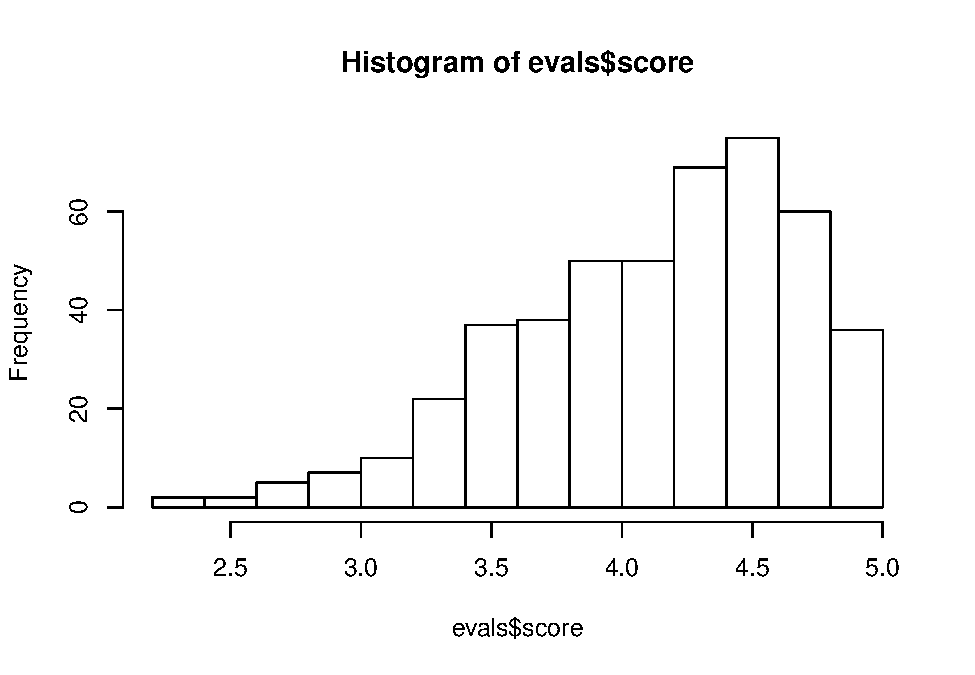
\includegraphics{multiple_regression_files/figure-latex/quest-2-1.pdf}
The distribution is unimodal, with a left skew, which means students
tend to give higher ratings. This is surprising to me, since research
has shown that people are more likely to leave a review when they are
dissatisfied.

\subsubsection{Question 3}\label{question-3}

Excluding \texttt{score}, select two other variables and describe their
relationship using an appropriate visualization (scatterplot,
side-by-side boxplots, or mosaic plot).

\paragraph{Solution}\label{solution-2}

\begin{Shaded}
\begin{Highlighting}[]
\KeywordTok{plot}\NormalTok{(evals}\OperatorTok{$}\NormalTok{cls_perc_eval }\OperatorTok{~}\StringTok{ }\NormalTok{evals}\OperatorTok{$}\NormalTok{gender)}
\end{Highlighting}
\end{Shaded}

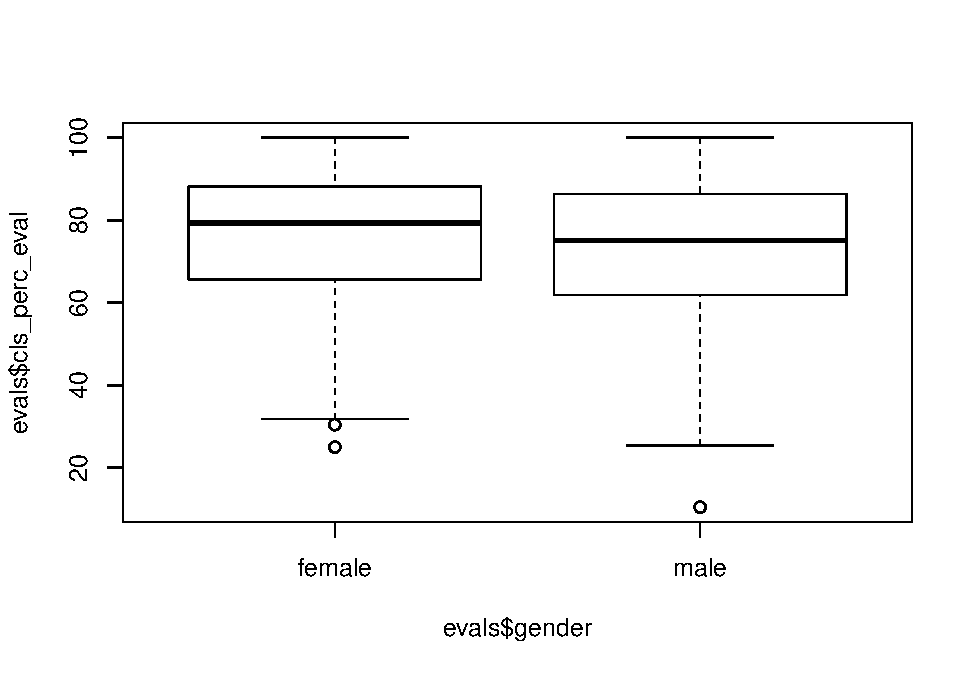
\includegraphics{multiple_regression_files/figure-latex/quest-3-1.pdf}

The percentage of the class that fills out the evaluation doesn't differ
too much based on the gender of the professor.

\subsection{Simple linear regression}\label{simple-linear-regression}

The fundamental phenomenon suggested by the study is that better looking
teachers are evaluated more favorably. Let's create a scatterplot to see
if this appears to be the case:

\begin{Shaded}
\begin{Highlighting}[]
\KeywordTok{plot}\NormalTok{(evals}\OperatorTok{$}\NormalTok{score }\OperatorTok{~}\StringTok{ }\NormalTok{evals}\OperatorTok{$}\NormalTok{bty_avg)}
\end{Highlighting}
\end{Shaded}

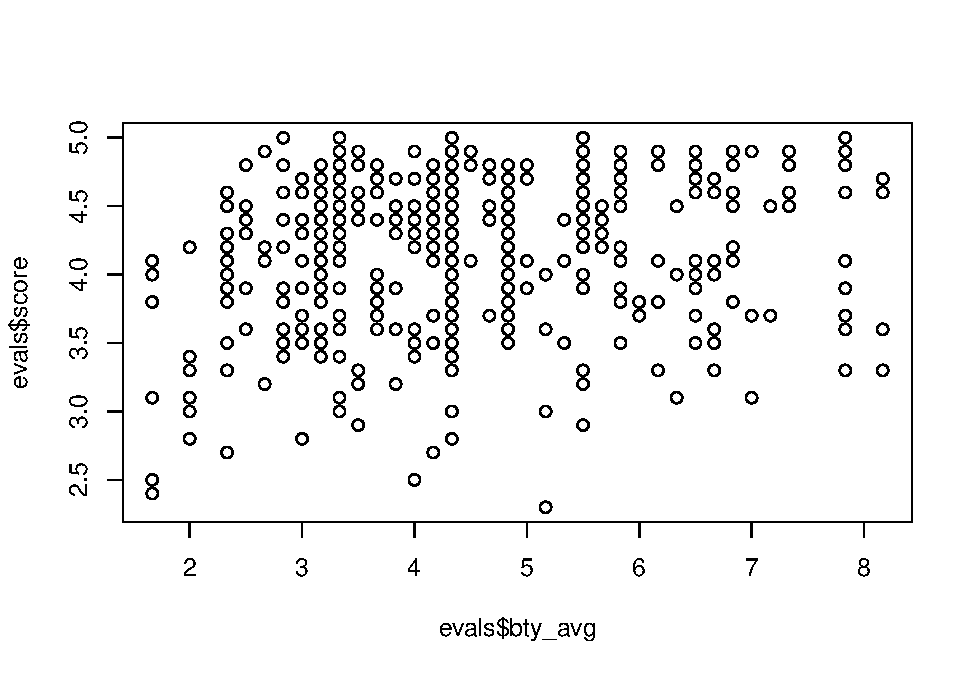
\includegraphics{multiple_regression_files/figure-latex/scatter-score-bty_avg-1.pdf}

Before we draw conclusions about the trend, compare the number of
observations in the data frame with the approximate number of points on
the scatterplot. Is anything awry?

There were 463 observations, but the scatterplot has fewer points.

\subsubsection{Question 4}\label{question-4}

Replot the scatterplot, but this time use the function \texttt{jitter()}
on the \(y\)- or the \(x\)-coordinate. (Use \texttt{?jitter} to learn
more.) What was misleading about the initial scatterplot?

\paragraph{Solution}\label{solution-3}

\begin{Shaded}
\begin{Highlighting}[]
\KeywordTok{plot}\NormalTok{(}\KeywordTok{jitter}\NormalTok{(evals}\OperatorTok{$}\NormalTok{score)}\OperatorTok{~}\NormalTok{evals}\OperatorTok{$}\NormalTok{bty_avg)}
\end{Highlighting}
\end{Shaded}

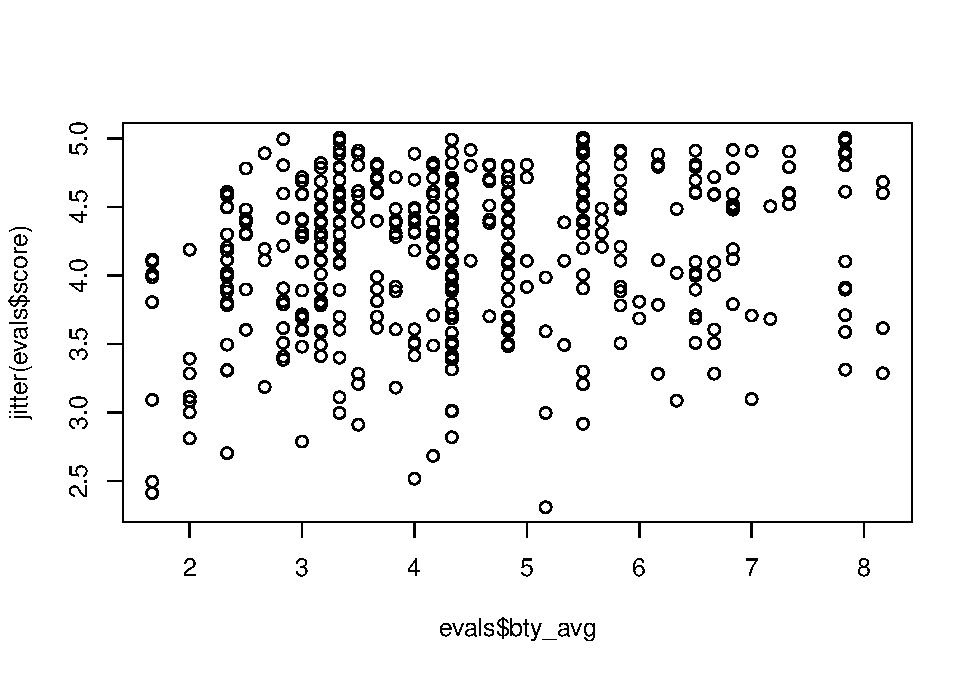
\includegraphics{multiple_regression_files/figure-latex/quest-4-1.pdf}

We can see that there are many points on top of each other, which is why
the scatterplot had fewer points.

\subsubsection{Question 5}\label{question-5}

Let's see if the apparent trend in the plot is something more than
natural variation. Fit a linear model called \texttt{m\_bty} to predict
average professor score by average beauty rating and add the line to
your plot using \texttt{abline(m\_bty)}. Write out the equation for the
linear model and interpret the slope. Is average beauty score a
statistically significant predictor? Does it appear to be a practically
significant predictor?

\paragraph{Solution}\label{solution-4}

\begin{Shaded}
\begin{Highlighting}[]
\NormalTok{m_bty <-}\StringTok{ }\KeywordTok{lm}\NormalTok{(score }\OperatorTok{~}\StringTok{ }\NormalTok{bty_avg, }\DataTypeTok{data =}\NormalTok{ evals)}
\KeywordTok{plot}\NormalTok{(}\KeywordTok{jitter}\NormalTok{(evals}\OperatorTok{$}\NormalTok{score) }\OperatorTok{~}\StringTok{ }\NormalTok{evals}\OperatorTok{$}\NormalTok{bty_avg)}
\KeywordTok{abline}\NormalTok{(m_bty)}
\end{Highlighting}
\end{Shaded}

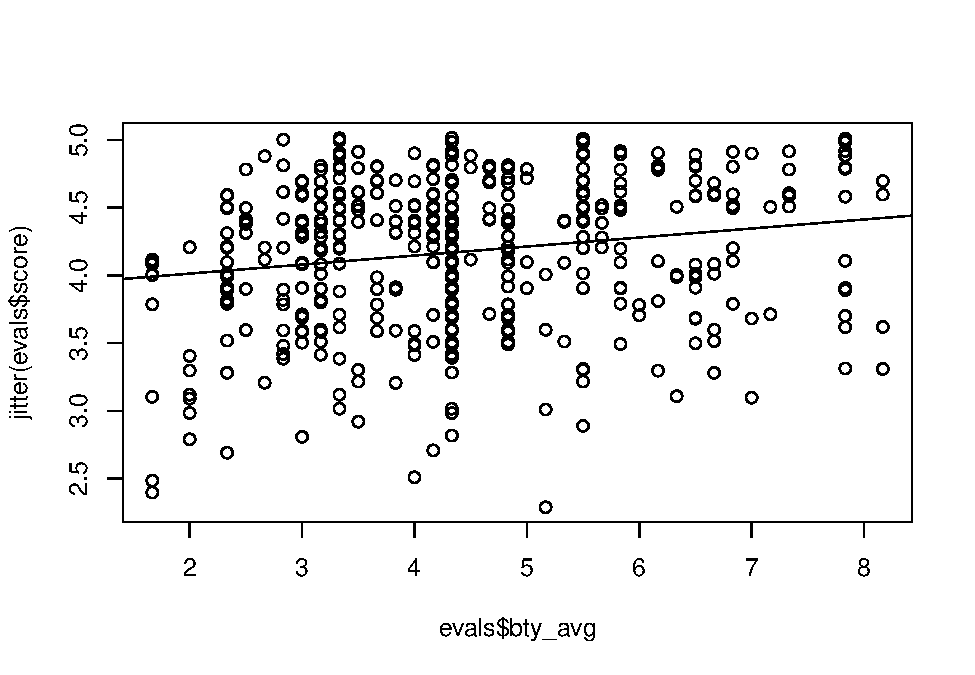
\includegraphics{multiple_regression_files/figure-latex/quest-5-1.pdf}

\begin{Shaded}
\begin{Highlighting}[]
\KeywordTok{summary}\NormalTok{(m_bty)}
\end{Highlighting}
\end{Shaded}

\begin{verbatim}
## 
## Call:
## lm(formula = score ~ bty_avg, data = evals)
## 
## Residuals:
##     Min      1Q  Median      3Q     Max 
## -1.9246 -0.3690  0.1420  0.3977  0.9309 
## 
## Coefficients:
##             Estimate Std. Error t value Pr(>|t|)    
## (Intercept)  3.88034    0.07614   50.96  < 2e-16 ***
## bty_avg      0.06664    0.01629    4.09 5.08e-05 ***
## ---
## Signif. codes:  0 '***' 0.001 '**' 0.01 '*' 0.05 '.' 0.1 ' ' 1
## 
## Residual standard error: 0.5348 on 461 degrees of freedom
## Multiple R-squared:  0.03502,    Adjusted R-squared:  0.03293 
## F-statistic: 16.73 on 1 and 461 DF,  p-value: 5.083e-05
\end{verbatim}

\(\widehat{score} =\) 3.880338 + 0.066637 \(\times \text{bty_avg}\)

Average beauty score is significant, since its p-value is nearly 0. It's
not a practically significant predictor, though, since every additional
point in \texttt{bty\_avg} results in 0.066637 additional points in
overall score.

\subsubsection{Question 6}\label{question-6}

Use residual plots to evaluate whether the conditions of least squares
regression are reasonable. Provide plots and comments for each one (see
the Simple Regression Lab for a reminder of how to make these).

\paragraph{Solution}\label{solution-5}

\begin{Shaded}
\begin{Highlighting}[]
\KeywordTok{plot}\NormalTok{(m_bty}\OperatorTok{$}\NormalTok{residuals }\OperatorTok{~}\StringTok{ }\NormalTok{evals}\OperatorTok{$}\NormalTok{bty_avg)}
\KeywordTok{abline}\NormalTok{(}\DataTypeTok{h =} \DecValTok{0}\NormalTok{, }\DataTypeTok{lty =} \DecValTok{3}\NormalTok{)}
\end{Highlighting}
\end{Shaded}

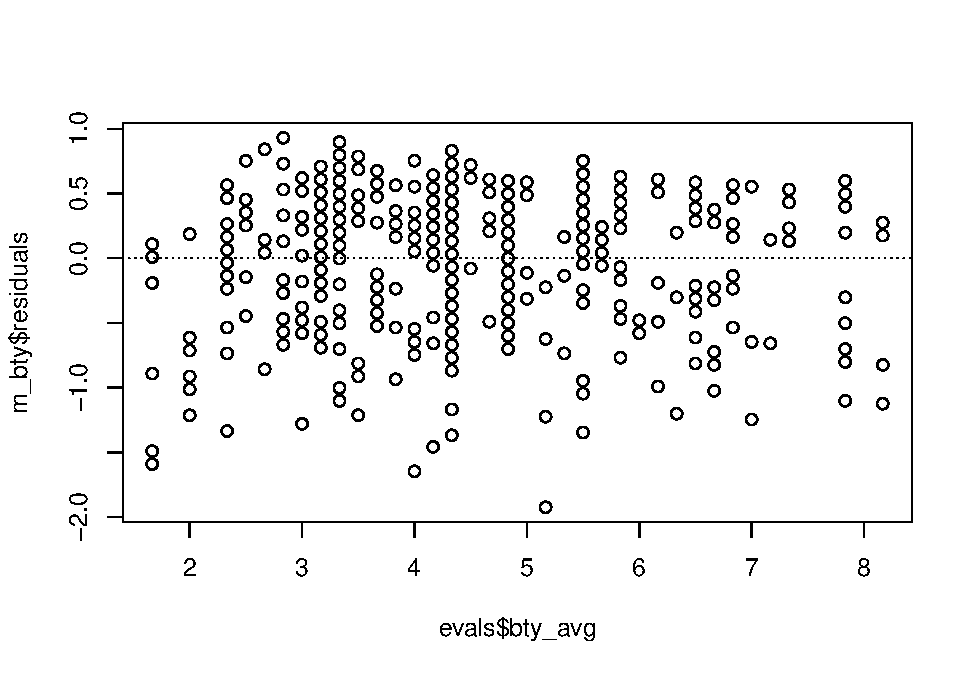
\includegraphics{multiple_regression_files/figure-latex/quest-6-1.pdf}

\begin{Shaded}
\begin{Highlighting}[]
\KeywordTok{hist}\NormalTok{(m_bty}\OperatorTok{$}\NormalTok{residuals)}
\end{Highlighting}
\end{Shaded}

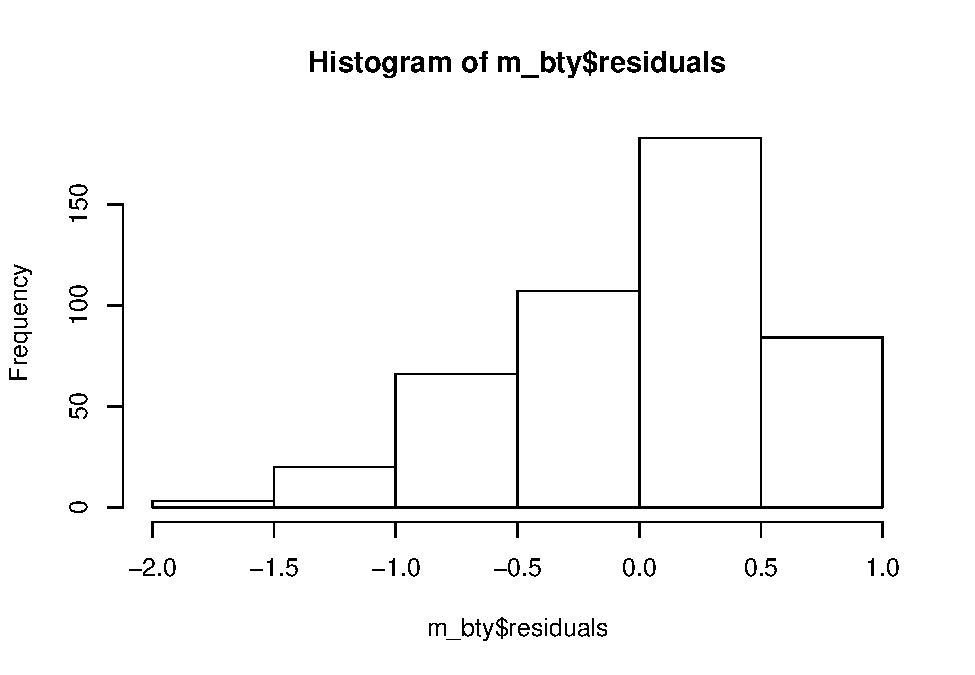
\includegraphics{multiple_regression_files/figure-latex/quest-6-2.pdf}

\begin{Shaded}
\begin{Highlighting}[]
\KeywordTok{qqnorm}\NormalTok{(m_bty}\OperatorTok{$}\NormalTok{residuals)}
\KeywordTok{qqline}\NormalTok{(m_bty}\OperatorTok{$}\NormalTok{residuals)}
\end{Highlighting}
\end{Shaded}

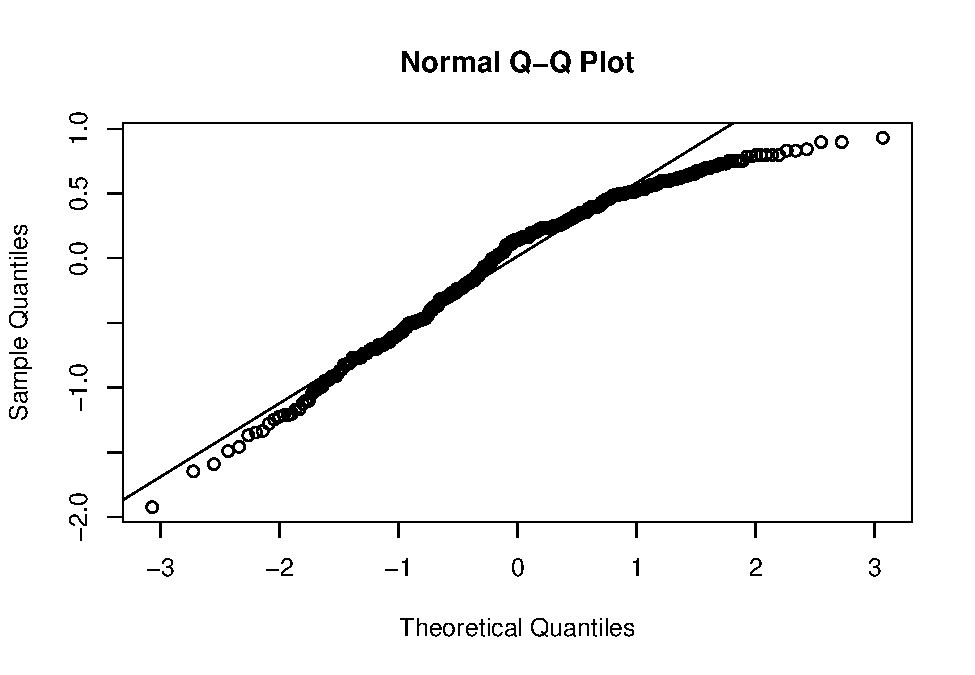
\includegraphics{multiple_regression_files/figure-latex/quest-6-3.pdf}

The histogram is left-skewed, and the plot does not follow the diagonal
line. Since the conditions for least squares regression are not met, we
cannot use it in this case.

\subsection{Multiple linear
regression}\label{multiple-linear-regression}

The data set contains several variables on the beauty score of the
professor: individual ratings from each of the six students who were
asked to score the physical appearance of the professors and the average
of these six scores. Let's take a look at the relationship between one
of these scores and the average beauty score.

\begin{Shaded}
\begin{Highlighting}[]
\KeywordTok{plot}\NormalTok{(evals}\OperatorTok{$}\NormalTok{bty_avg }\OperatorTok{~}\StringTok{ }\NormalTok{evals}\OperatorTok{$}\NormalTok{bty_f1lower)}
\end{Highlighting}
\end{Shaded}

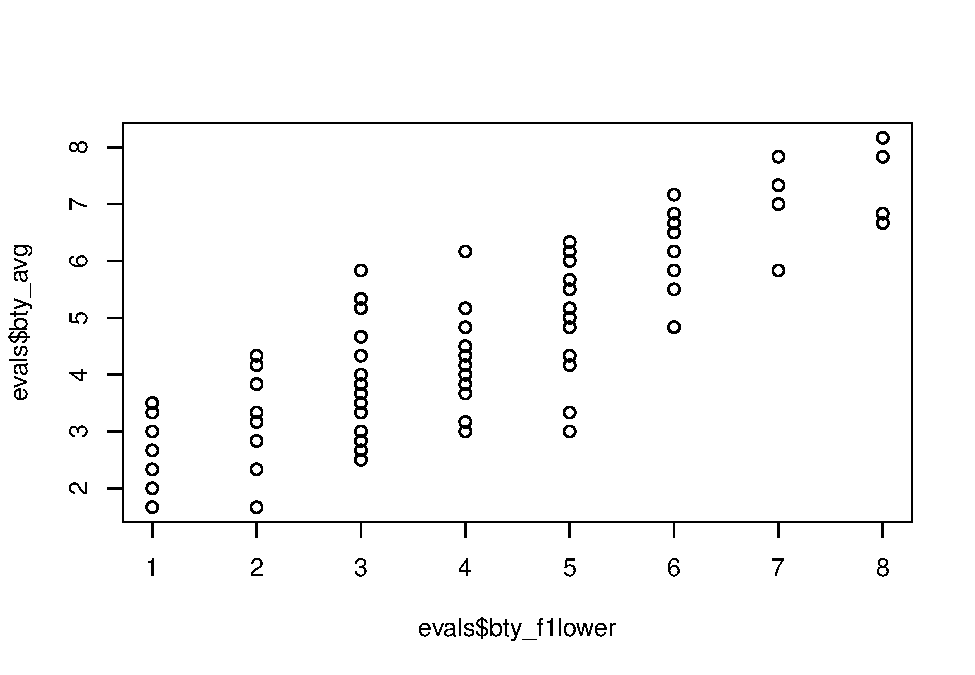
\includegraphics{multiple_regression_files/figure-latex/bty-rel-1.pdf}

\begin{Shaded}
\begin{Highlighting}[]
\KeywordTok{cor}\NormalTok{(evals}\OperatorTok{$}\NormalTok{bty_avg, evals}\OperatorTok{$}\NormalTok{bty_f1lower)}
\end{Highlighting}
\end{Shaded}

\begin{verbatim}
## [1] 0.8439112
\end{verbatim}

As expected the relationship is quite strong - after all, the average
score is calculated using the individual scores. We can actually take a
look at the relationships between all beauty variables (columns 13
through 19) using the following command:

\begin{Shaded}
\begin{Highlighting}[]
\KeywordTok{plot}\NormalTok{(evals[,}\DecValTok{13}\OperatorTok{:}\DecValTok{19}\NormalTok{])}
\end{Highlighting}
\end{Shaded}

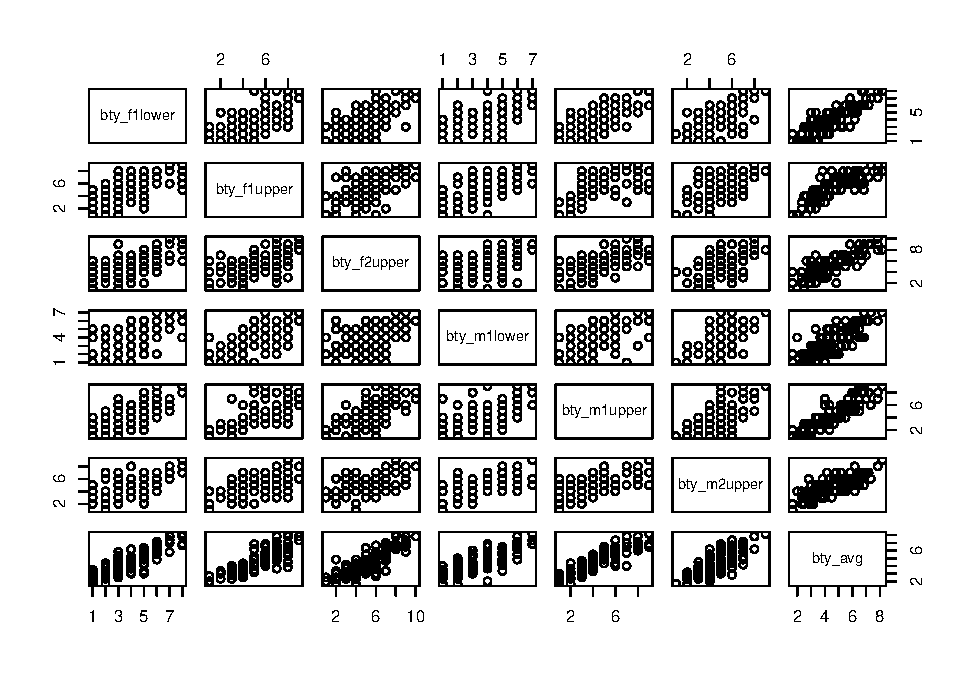
\includegraphics{multiple_regression_files/figure-latex/bty-rels-1.pdf}

These variables are collinear (correlated), and adding more than one of
these variables to the model would not add much value to the model. In
this application and with these highly-correlated predictors, it is
reasonable to use the average beauty score as the single representative
of these variables.

In order to see if beauty is still a significant predictor of professor
score after we've accounted for the gender of the professor, we can add
the gender term into the model.

\begin{Shaded}
\begin{Highlighting}[]
\NormalTok{m_bty_gen <-}\StringTok{ }\KeywordTok{lm}\NormalTok{(score }\OperatorTok{~}\StringTok{ }\NormalTok{bty_avg }\OperatorTok{+}\StringTok{ }\NormalTok{gender, }\DataTypeTok{data =}\NormalTok{ evals)}
\KeywordTok{summary}\NormalTok{(m_bty_gen)}
\end{Highlighting}
\end{Shaded}

\begin{verbatim}
## 
## Call:
## lm(formula = score ~ bty_avg + gender, data = evals)
## 
## Residuals:
##     Min      1Q  Median      3Q     Max 
## -1.8305 -0.3625  0.1055  0.4213  0.9314 
## 
## Coefficients:
##             Estimate Std. Error t value Pr(>|t|)    
## (Intercept)  3.74734    0.08466  44.266  < 2e-16 ***
## bty_avg      0.07416    0.01625   4.563 6.48e-06 ***
## gendermale   0.17239    0.05022   3.433 0.000652 ***
## ---
## Signif. codes:  0 '***' 0.001 '**' 0.01 '*' 0.05 '.' 0.1 ' ' 1
## 
## Residual standard error: 0.5287 on 460 degrees of freedom
## Multiple R-squared:  0.05912,    Adjusted R-squared:  0.05503 
## F-statistic: 14.45 on 2 and 460 DF,  p-value: 8.177e-07
\end{verbatim}

\subsubsection{Question 7}\label{question-7}

P-values and parameter estimates should only be trusted if the
conditions for the regression are reasonable. Verify that the conditions
for this model are reasonable using diagnostic plots.

\paragraph{Solution}\label{solution-6}

\begin{Shaded}
\begin{Highlighting}[]
\KeywordTok{plot}\NormalTok{(m_bty_gen}\OperatorTok{$}\NormalTok{residuals }\OperatorTok{~}\StringTok{ }\NormalTok{evals}\OperatorTok{$}\NormalTok{bty_avg)}
\KeywordTok{abline}\NormalTok{(}\DataTypeTok{h =} \DecValTok{0}\NormalTok{, }\DataTypeTok{lty =} \DecValTok{3}\NormalTok{)}
\end{Highlighting}
\end{Shaded}

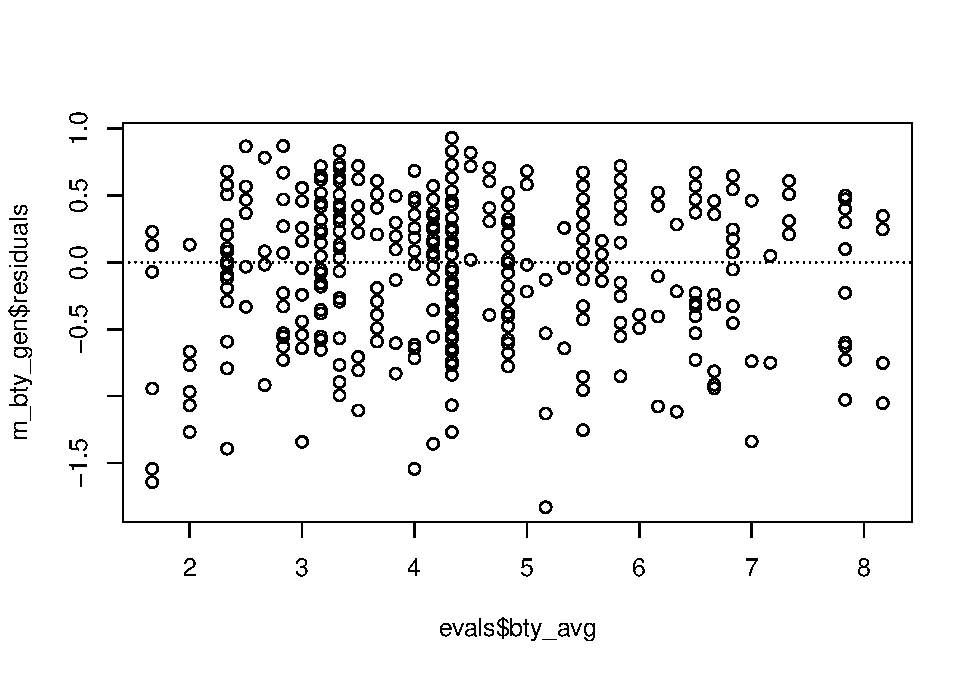
\includegraphics{multiple_regression_files/figure-latex/quest-7-1.pdf}

\begin{Shaded}
\begin{Highlighting}[]
\KeywordTok{hist}\NormalTok{(m_bty_gen}\OperatorTok{$}\NormalTok{residuals)}
\end{Highlighting}
\end{Shaded}

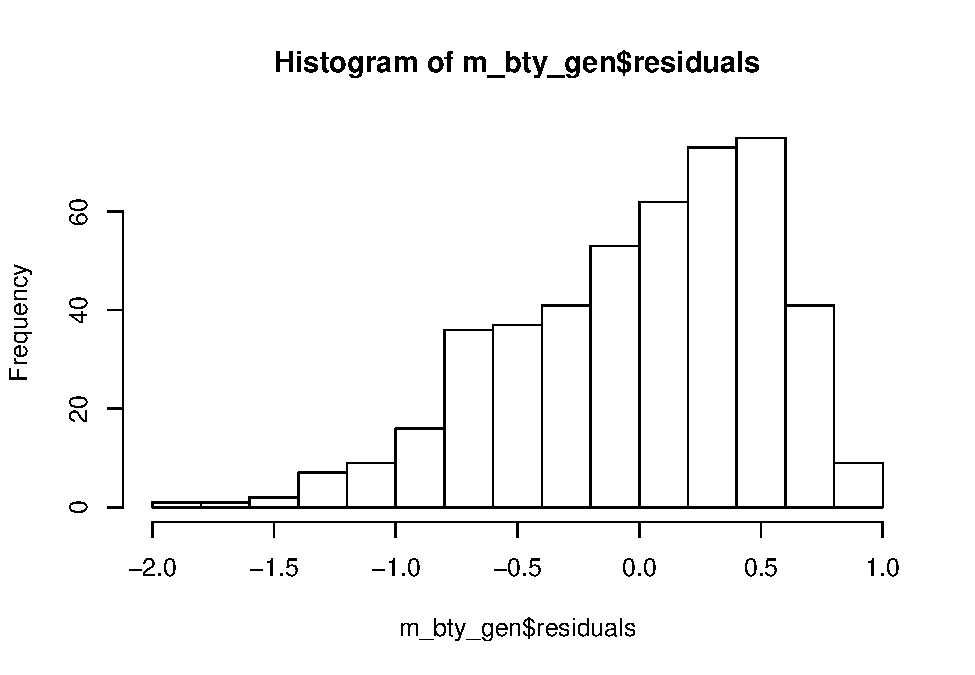
\includegraphics{multiple_regression_files/figure-latex/quest-7-2.pdf}

\begin{Shaded}
\begin{Highlighting}[]
\KeywordTok{qqnorm}\NormalTok{(m_bty_gen}\OperatorTok{$}\NormalTok{residuals)}
\KeywordTok{qqline}\NormalTok{(m_bty_gen}\OperatorTok{$}\NormalTok{residuals)}
\end{Highlighting}
\end{Shaded}

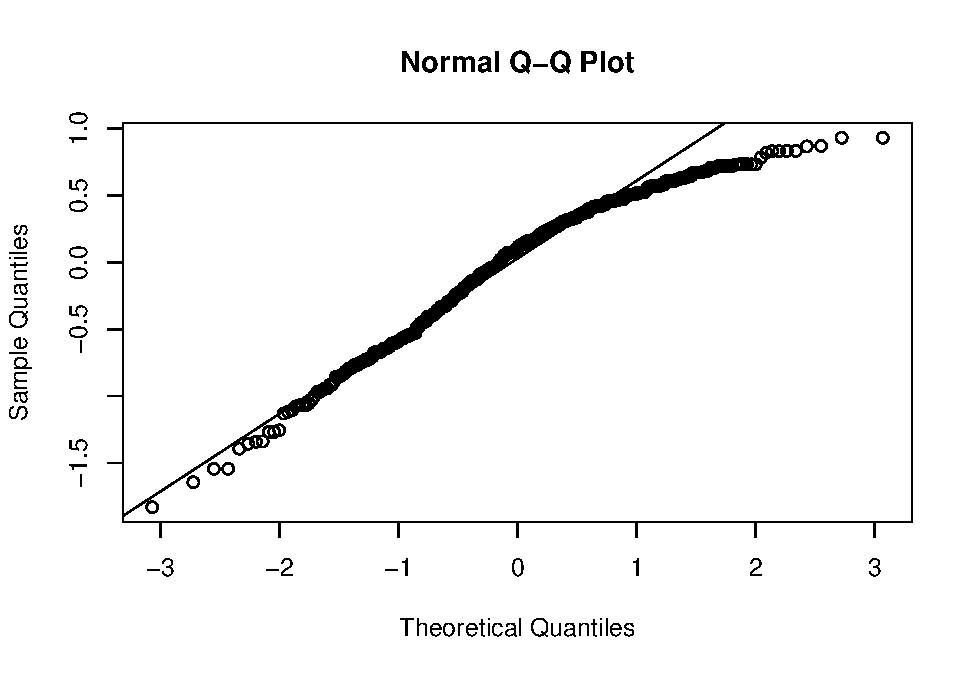
\includegraphics{multiple_regression_files/figure-latex/quest-7-3.pdf}
The histogram is left-skewed, and the plot does not follow the diagonal
line. The conditions for least square regression are not met, and it
cannot be used in this case.

\subsubsection{Question 8}\label{question-8}

Is \texttt{bty\_avg} still a significant predictor of \texttt{score}?
Has the addition of \texttt{gender} to the model changed the parameter
estimate for \texttt{bty\_avg}?

\paragraph{Solution}\label{solution-7}

The addition of \texttt{gender} has reduced the p-value even further,
making \texttt{bty\_avg} an even more significant predictor.

Note that the estimate for \texttt{gender} is now called
\texttt{gendermale}. You'll see this name change whenever you introduce
a categorical variable. The reason is that R recodes \texttt{gender}
from having the values of \texttt{female} and \texttt{male} to being an
indicator variable called \texttt{gendermale} that takes a value of
\(0\) for females and a value of \(1\) for males. (Such variables are
often referred to as ``dummy'' variables.)

As a result, for females, the parameter estimate is multiplied by zero,
leaving the intercept and slope form familiar from simple regression.

\[
  \begin{aligned}
\widehat{score} &= \hat{\beta}_0 + \hat{\beta}_1 \times bty\_avg + \hat{\beta}_2 \times (0) \\
&= \hat{\beta}_0 + \hat{\beta}_1 \times bty\_avg\end{aligned}
\]

We can plot this line and the line corresponding to males with the
following custom function.

\begin{Shaded}
\begin{Highlighting}[]
\KeywordTok{multiLines}\NormalTok{(m_bty_gen)}
\end{Highlighting}
\end{Shaded}

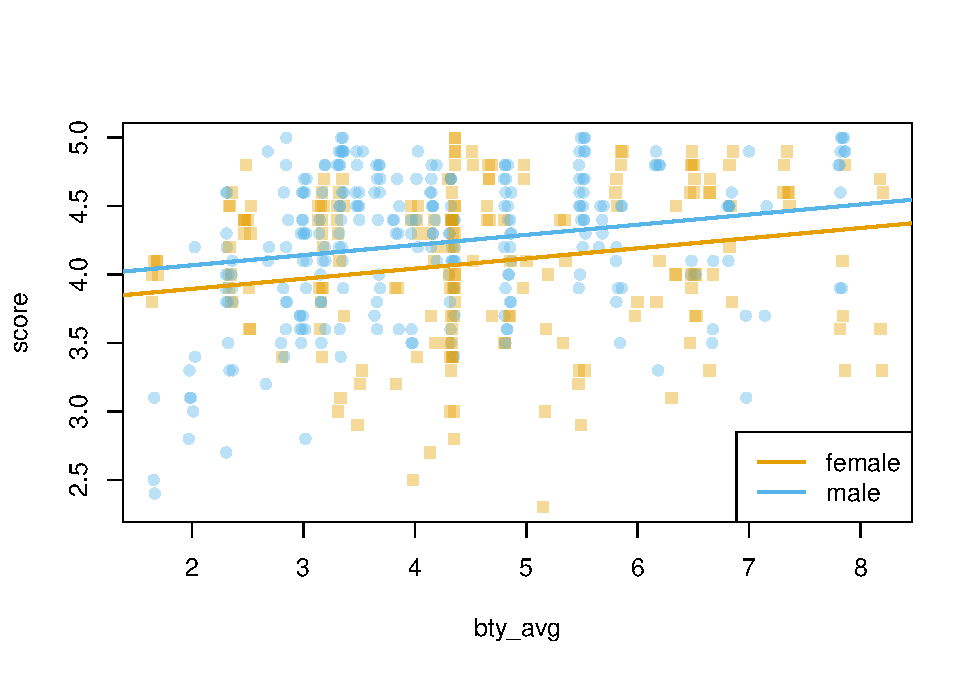
\includegraphics{multiple_regression_files/figure-latex/twoLines-1.pdf}

\subsubsection{Question 9}\label{question-9}

What is the equation of the line corresponding to males? (\emph{Hint:}
For males, the parameter estimate is multiplied by 1.) For two
professors who received the same beauty rating, which gender tends to
have the higher course evaluation score?

\paragraph{Solution}\label{solution-8}

\(\widehat{score} = \hat{\beta_0} + \hat{\beta_1} \times \text{bty_avg} + \hat{\beta_2} \times \text{Male}\)
\(\widehat{score} = 3.7473382 + 0.0741554 \times \text{bty_avg} + 0.1723895 \times 1\)
\(\widehat{score} = 3.9197278 + 0.0741554 \times \text{bty_avg}\).

Of the two professors with the same beauty rating, the male's evaluation
score will be higher by 0.1723895.

The decision to call the indicator variable \texttt{gendermale} instead
of\texttt{genderfemale} has no deeper meaning. R simply codes the
category that comes first alphabetically as a \(0\). (You can change the
reference level of a categorical variable, which is the level that is
coded as a 0, using the\texttt{relevel} function. Use \texttt{?relevel}
to learn more.)

\subsubsection{Question 10}\label{question-10}

Create a new model called \texttt{m\_bty\_rank} with \texttt{gender}
removed and \texttt{rank} added in. How does R appear to handle
categorical variables that have more than two levels? Note that the rank
variable has three levels: \texttt{teaching}, \texttt{tenure\ track},
\texttt{tenured}.

\paragraph{Solution}\label{solution-9}

\begin{Shaded}
\begin{Highlighting}[]
\NormalTok{m_bty_rank <-}\StringTok{ }\KeywordTok{lm}\NormalTok{(score }\OperatorTok{~}\StringTok{ }\NormalTok{bty_avg }\OperatorTok{+}\StringTok{ }\NormalTok{rank, }\DataTypeTok{data =}\NormalTok{ evals)}
\KeywordTok{summary}\NormalTok{(m_bty_rank)}
\end{Highlighting}
\end{Shaded}

\begin{verbatim}
## 
## Call:
## lm(formula = score ~ bty_avg + rank, data = evals)
## 
## Residuals:
##     Min      1Q  Median      3Q     Max 
## -1.8713 -0.3642  0.1489  0.4103  0.9525 
## 
## Coefficients:
##                  Estimate Std. Error t value Pr(>|t|)    
## (Intercept)       3.98155    0.09078  43.860  < 2e-16 ***
## bty_avg           0.06783    0.01655   4.098 4.92e-05 ***
## ranktenure track -0.16070    0.07395  -2.173   0.0303 *  
## ranktenured      -0.12623    0.06266  -2.014   0.0445 *  
## ---
## Signif. codes:  0 '***' 0.001 '**' 0.01 '*' 0.05 '.' 0.1 ' ' 1
## 
## Residual standard error: 0.5328 on 459 degrees of freedom
## Multiple R-squared:  0.04652,    Adjusted R-squared:  0.04029 
## F-statistic: 7.465 on 3 and 459 DF,  p-value: 6.88e-05
\end{verbatim}

\begin{Shaded}
\begin{Highlighting}[]
\KeywordTok{multiLines}\NormalTok{(m_bty_rank)}
\end{Highlighting}
\end{Shaded}

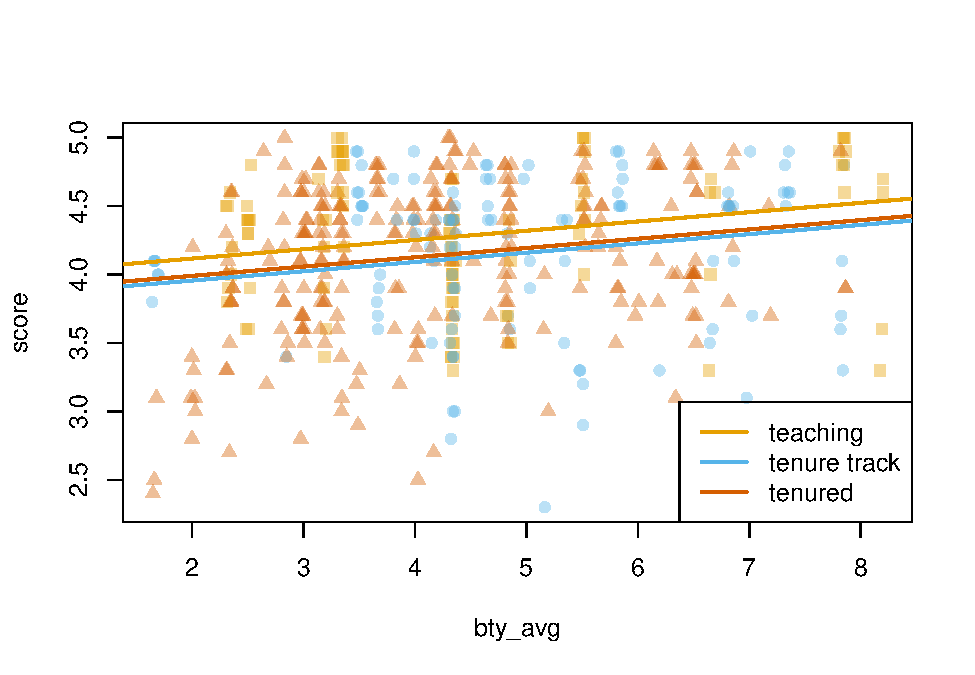
\includegraphics{multiple_regression_files/figure-latex/quest-10-1.pdf}
R creates dummy variables for each level.

The interpretation of the coefficients in multiple regression is
slightly different from that of simple regression. The estimate for
\texttt{bty\_avg} reflects how much higher a group of professors is
expected to score if they have a beauty rating that is one point higher
\emph{while holding all other variables constant}. In this case, that
translates into considering only professors of the same rank with
\texttt{bty\_avg} scores that are one point apart.

\subsection{The search for the best
model}\label{the-search-for-the-best-model}

We will start with a full model that predicts professor score based on
rank, ethnicity, gender, language of the university where they got their
degree, age, proportion of students that filled out evaluations, class
size, course level, number of professors, number of credits, average
beauty rating, outfit, and picture color.

\subsubsection{Question 11}\label{question-11}

Which variable would you expect to have the highest p-value in this
model? Why? \emph{Hint:} Think about which variable would you expect to
not have any association with the professor score.

\paragraph{Solution}\label{solution-10}

I would guess \texttt{language} would have the least impact.

Let's run the model\ldots{}

\begin{Shaded}
\begin{Highlighting}[]
\NormalTok{m_full <-}\StringTok{ }\KeywordTok{lm}\NormalTok{(score }\OperatorTok{~}\StringTok{ }\NormalTok{rank }\OperatorTok{+}\StringTok{ }\NormalTok{ethnicity }\OperatorTok{+}\StringTok{ }\NormalTok{gender }\OperatorTok{+}\StringTok{ }\NormalTok{language }\OperatorTok{+}\StringTok{ }\NormalTok{age }\OperatorTok{+}\StringTok{ }\NormalTok{cls_perc_eval }
             \OperatorTok{+}\StringTok{ }\NormalTok{cls_students }\OperatorTok{+}\StringTok{ }\NormalTok{cls_level }\OperatorTok{+}\StringTok{ }\NormalTok{cls_profs }\OperatorTok{+}\StringTok{ }\NormalTok{cls_credits }\OperatorTok{+}\StringTok{ }\NormalTok{bty_avg }
             \OperatorTok{+}\StringTok{ }\NormalTok{pic_outfit }\OperatorTok{+}\StringTok{ }\NormalTok{pic_color, }\DataTypeTok{data =}\NormalTok{ evals)}
\KeywordTok{summary}\NormalTok{(m_full)}
\end{Highlighting}
\end{Shaded}

\begin{verbatim}
## 
## Call:
## lm(formula = score ~ rank + ethnicity + gender + language + age + 
##     cls_perc_eval + cls_students + cls_level + cls_profs + cls_credits + 
##     bty_avg + pic_outfit + pic_color, data = evals)
## 
## Residuals:
##      Min       1Q   Median       3Q      Max 
## -1.77397 -0.32432  0.09067  0.35183  0.95036 
## 
## Coefficients:
##                         Estimate Std. Error t value Pr(>|t|)    
## (Intercept)            4.0952141  0.2905277  14.096  < 2e-16 ***
## ranktenure track      -0.1475932  0.0820671  -1.798  0.07278 .  
## ranktenured           -0.0973378  0.0663296  -1.467  0.14295    
## ethnicitynot minority  0.1234929  0.0786273   1.571  0.11698    
## gendermale             0.2109481  0.0518230   4.071 5.54e-05 ***
## languagenon-english   -0.2298112  0.1113754  -2.063  0.03965 *  
## age                   -0.0090072  0.0031359  -2.872  0.00427 ** 
## cls_perc_eval          0.0053272  0.0015393   3.461  0.00059 ***
## cls_students           0.0004546  0.0003774   1.205  0.22896    
## cls_levelupper         0.0605140  0.0575617   1.051  0.29369    
## cls_profssingle       -0.0146619  0.0519885  -0.282  0.77806    
## cls_creditsone credit  0.5020432  0.1159388   4.330 1.84e-05 ***
## bty_avg                0.0400333  0.0175064   2.287  0.02267 *  
## pic_outfitnot formal  -0.1126817  0.0738800  -1.525  0.12792    
## pic_colorcolor        -0.2172630  0.0715021  -3.039  0.00252 ** 
## ---
## Signif. codes:  0 '***' 0.001 '**' 0.01 '*' 0.05 '.' 0.1 ' ' 1
## 
## Residual standard error: 0.498 on 448 degrees of freedom
## Multiple R-squared:  0.1871, Adjusted R-squared:  0.1617 
## F-statistic: 7.366 on 14 and 448 DF,  p-value: 6.552e-14
\end{verbatim}

\subsubsection{Question 12}\label{question-12}

Check your suspicions from the previous exercise. Include the model
output in your response.

\paragraph{Solution}\label{solution-11}

The variable with the highest p-value is \texttt{cls\_profs} with
0.77806, compared to 0.03965 for \texttt{language}. I guessed wrong.

\subsubsection{Question 13}\label{question-13}

Interpret the coefficient associated with the ethnicity variable.

\paragraph{Solution}\label{solution-12}

Keeping all other variables constant, professors that are not a minority
will have a score higher by 0.1234929.

\subsubsection{Question 14}\label{question-14}

Drop the variable with the highest p-value and re-fit the model. Did the
coefficients and significance of the other explanatory variables change?
(One of the things that makes multiple regression interesting is that
coefficient estimates depend on the other variables that are included in
the model.) If not, what does this say about whether or not the dropped
variable was collinear with the other explanatory variables?

\paragraph{Solution}\label{solution-13}

\begin{Shaded}
\begin{Highlighting}[]
\NormalTok{m_full_refit <-}\StringTok{ }\KeywordTok{lm}\NormalTok{(score }\OperatorTok{~}\StringTok{ }\NormalTok{rank }\OperatorTok{+}\StringTok{ }\NormalTok{ethnicity }\OperatorTok{+}\StringTok{ }\NormalTok{gender }\OperatorTok{+}\StringTok{ }\NormalTok{language }\OperatorTok{+}\StringTok{ }\NormalTok{age }\OperatorTok{+}\StringTok{ }\NormalTok{cls_perc_eval }
             \OperatorTok{+}\StringTok{ }\NormalTok{cls_students }\OperatorTok{+}\StringTok{ }\NormalTok{cls_level }\OperatorTok{+}\StringTok{ }\NormalTok{cls_credits }\OperatorTok{+}\StringTok{ }\NormalTok{bty_avg }
             \OperatorTok{+}\StringTok{ }\NormalTok{pic_outfit }\OperatorTok{+}\StringTok{ }\NormalTok{pic_color, }\DataTypeTok{data =}\NormalTok{ evals)}
\KeywordTok{summary}\NormalTok{(m_full_refit)}
\end{Highlighting}
\end{Shaded}

\begin{verbatim}
## 
## Call:
## lm(formula = score ~ rank + ethnicity + gender + language + age + 
##     cls_perc_eval + cls_students + cls_level + cls_credits + 
##     bty_avg + pic_outfit + pic_color, data = evals)
## 
## Residuals:
##     Min      1Q  Median      3Q     Max 
## -1.7836 -0.3257  0.0859  0.3513  0.9551 
## 
## Coefficients:
##                         Estimate Std. Error t value Pr(>|t|)    
## (Intercept)            4.0872523  0.2888562  14.150  < 2e-16 ***
## ranktenure track      -0.1476746  0.0819824  -1.801 0.072327 .  
## ranktenured           -0.0973829  0.0662614  -1.470 0.142349    
## ethnicitynot minority  0.1274458  0.0772887   1.649 0.099856 .  
## gendermale             0.2101231  0.0516873   4.065 5.66e-05 ***
## languagenon-english   -0.2282894  0.1111305  -2.054 0.040530 *  
## age                   -0.0089992  0.0031326  -2.873 0.004262 ** 
## cls_perc_eval          0.0052888  0.0015317   3.453 0.000607 ***
## cls_students           0.0004687  0.0003737   1.254 0.210384    
## cls_levelupper         0.0606374  0.0575010   1.055 0.292200    
## cls_creditsone credit  0.5061196  0.1149163   4.404 1.33e-05 ***
## bty_avg                0.0398629  0.0174780   2.281 0.023032 *  
## pic_outfitnot formal  -0.1083227  0.0721711  -1.501 0.134080    
## pic_colorcolor        -0.2190527  0.0711469  -3.079 0.002205 ** 
## ---
## Signif. codes:  0 '***' 0.001 '**' 0.01 '*' 0.05 '.' 0.1 ' ' 1
## 
## Residual standard error: 0.4974 on 449 degrees of freedom
## Multiple R-squared:  0.187,  Adjusted R-squared:  0.1634 
## F-statistic: 7.943 on 13 and 449 DF,  p-value: 2.336e-14
\end{verbatim}

Yes, the coefficients and significance of the other variables did
change, but not much, implying there wasn't much dependence between the
other variables and \texttt{cls\_profs}.

\subsubsection{Question 15}\label{question-15}

Using backward-selection and p-value as the selection criterion,
determine the best model. You do not need to show all steps in your
answer, just the output for the final model. Also, write out the linear
model for predicting score based on the final model you settle on.

\paragraph{Solution}\label{solution-14}

\begin{Shaded}
\begin{Highlighting}[]
\NormalTok{m_full_best <-}\StringTok{ }\KeywordTok{lm}\NormalTok{(score }\OperatorTok{~}\StringTok{ }\NormalTok{ethnicity }\OperatorTok{+}\StringTok{ }\NormalTok{gender }\OperatorTok{+}\StringTok{ }\NormalTok{language }\OperatorTok{+}\StringTok{ }\NormalTok{age }\OperatorTok{+}\StringTok{ }\NormalTok{cls_perc_eval }
             \OperatorTok{+}\StringTok{ }\NormalTok{cls_credits }\OperatorTok{+}\StringTok{ }\NormalTok{bty_avg }\OperatorTok{+}\StringTok{ }\NormalTok{pic_color, }\DataTypeTok{data =}\NormalTok{ evals)}
\KeywordTok{summary}\NormalTok{(m_full_best)}
\end{Highlighting}
\end{Shaded}

\begin{verbatim}
## 
## Call:
## lm(formula = score ~ ethnicity + gender + language + age + cls_perc_eval + 
##     cls_credits + bty_avg + pic_color, data = evals)
## 
## Residuals:
##      Min       1Q   Median       3Q      Max 
## -1.85320 -0.32394  0.09984  0.37930  0.93610 
## 
## Coefficients:
##                        Estimate Std. Error t value Pr(>|t|)    
## (Intercept)            3.771922   0.232053  16.255  < 2e-16 ***
## ethnicitynot minority  0.167872   0.075275   2.230  0.02623 *  
## gendermale             0.207112   0.050135   4.131 4.30e-05 ***
## languagenon-english   -0.206178   0.103639  -1.989  0.04726 *  
## age                   -0.006046   0.002612  -2.315  0.02108 *  
## cls_perc_eval          0.004656   0.001435   3.244  0.00127 ** 
## cls_creditsone credit  0.505306   0.104119   4.853 1.67e-06 ***
## bty_avg                0.051069   0.016934   3.016  0.00271 ** 
## pic_colorcolor        -0.190579   0.067351  -2.830  0.00487 ** 
## ---
## Signif. codes:  0 '***' 0.001 '**' 0.01 '*' 0.05 '.' 0.1 ' ' 1
## 
## Residual standard error: 0.4992 on 454 degrees of freedom
## Multiple R-squared:  0.1722, Adjusted R-squared:  0.1576 
## F-statistic:  11.8 on 8 and 454 DF,  p-value: 2.58e-15
\end{verbatim}

\begin{Shaded}
\begin{Highlighting}[]
\NormalTok{sumco.}\DecValTok{2}\NormalTok{ <-}\StringTok{ }\KeywordTok{summary}\NormalTok{(m_full_best)}\OperatorTok{$}\NormalTok{coefficients}
\end{Highlighting}
\end{Shaded}

Removed all variables with a p-value higher than 0.05.

\$ \widehat{score} = 3.7719215 + 0.1678723 \times \text{ethnicity} +
0.2071121 \times \text{gender}\$ \textbackslash{}
\(-0.2061781 \times \text{language}-0.0060459 \times \text{age} + 0.0046559 \times \text{cls_perc_eval}\)
\textbackslash{}
\(+ 0.5053062 \times \text{cls_credits} + 0.0510693 \times \text{bty_avg} -0.1905788 \times \text{pic_color}\)

\subsubsection{Question 16}\label{question-16}

Verify that the conditions for this model are reasonable using
diagnostic plots.

\paragraph{Solution}\label{solution-15}

\begin{Shaded}
\begin{Highlighting}[]
\KeywordTok{plot}\NormalTok{(m_full_best}\OperatorTok{$}\NormalTok{residuals }\OperatorTok{~}\StringTok{ }\NormalTok{evals}\OperatorTok{$}\NormalTok{bty_avg)}
\KeywordTok{abline}\NormalTok{(}\DataTypeTok{h =} \DecValTok{0}\NormalTok{, }\DataTypeTok{lty =} \DecValTok{3}\NormalTok{)}
\end{Highlighting}
\end{Shaded}

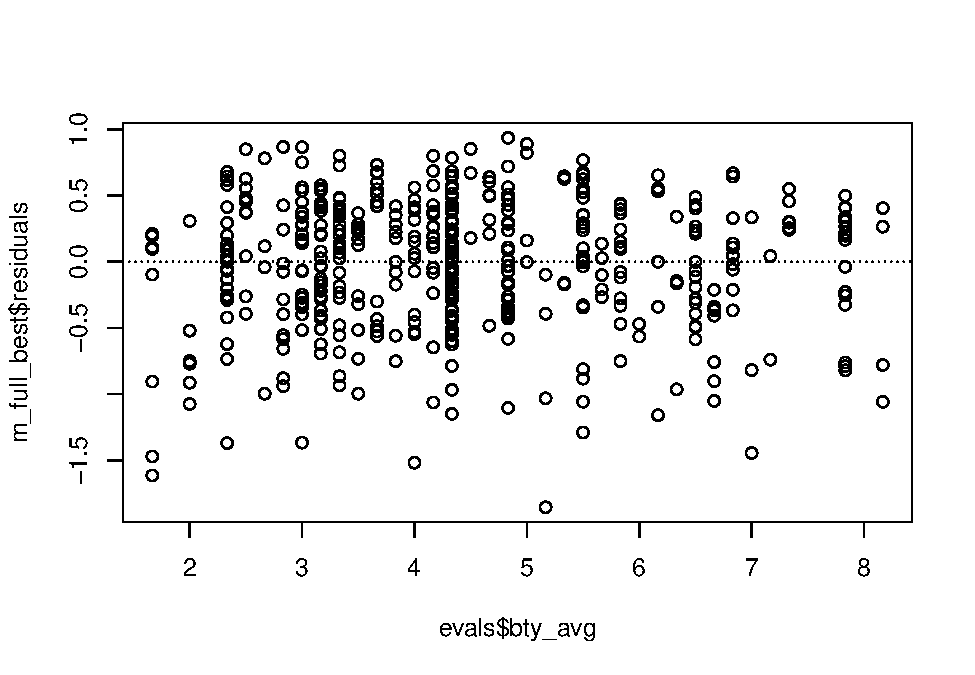
\includegraphics{multiple_regression_files/figure-latex/quest-16-1.pdf}

\begin{Shaded}
\begin{Highlighting}[]
\KeywordTok{hist}\NormalTok{(m_full_best}\OperatorTok{$}\NormalTok{residuals)}
\end{Highlighting}
\end{Shaded}

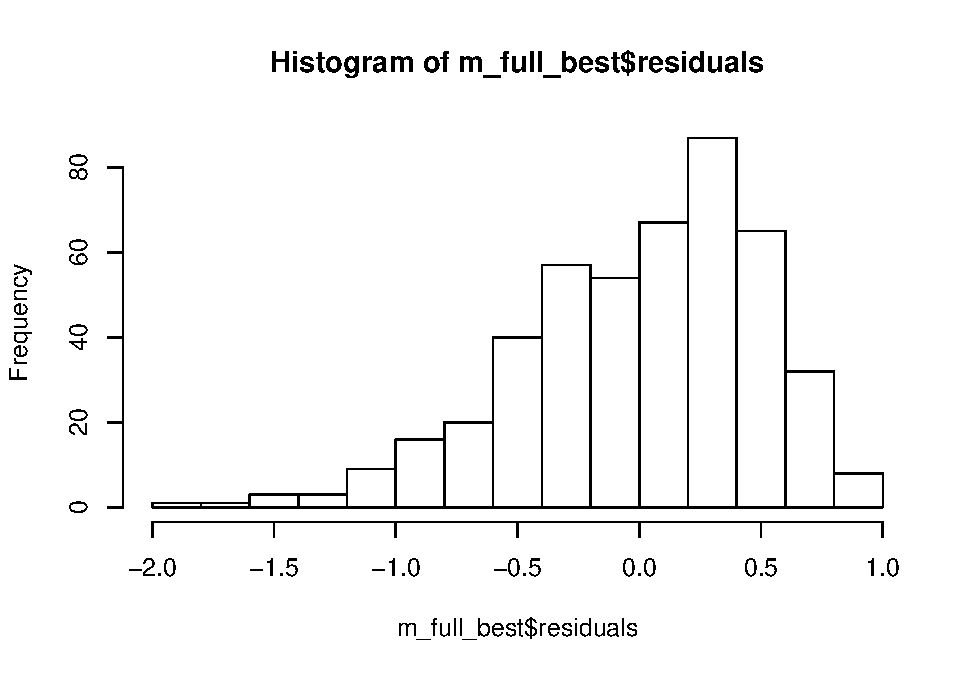
\includegraphics{multiple_regression_files/figure-latex/quest-16-2.pdf}

\begin{Shaded}
\begin{Highlighting}[]
\KeywordTok{qqnorm}\NormalTok{(m_full_best}\OperatorTok{$}\NormalTok{residuals)}
\KeywordTok{qqline}\NormalTok{(m_full_best}\OperatorTok{$}\NormalTok{residuals)}
\end{Highlighting}
\end{Shaded}

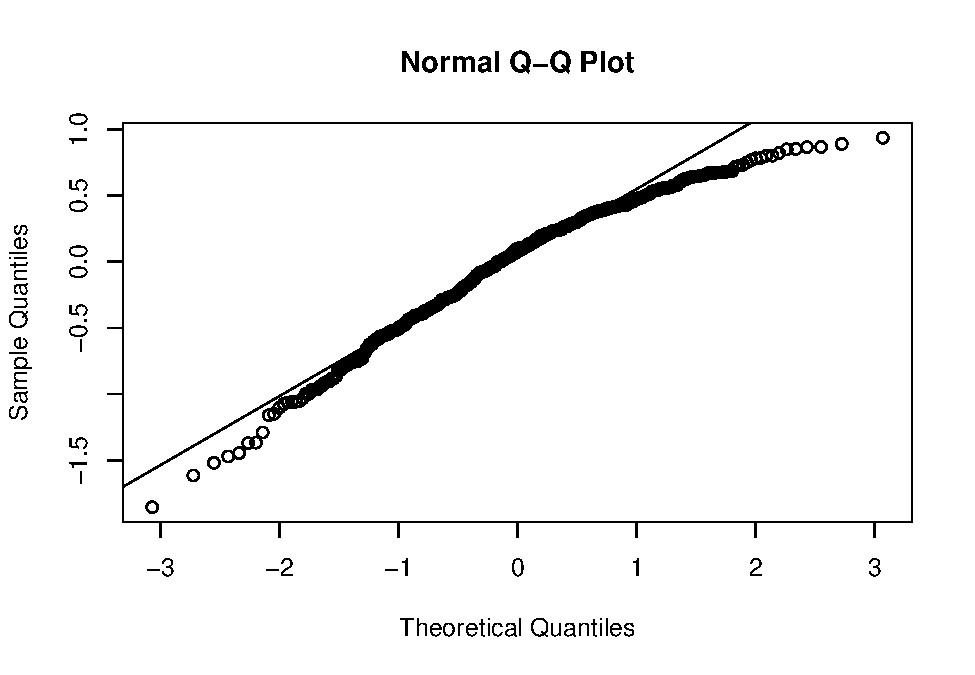
\includegraphics{multiple_regression_files/figure-latex/quest-16-3.pdf}
The histogram is left-skewed and the plot does not follow the diagonal
line. The residuals do not appear to be nearly normal.

\subsubsection{Question 17}\label{question-17}

The original paper describes how these data were gathered by taking a
sample of professors from the University of Texas at Austin and
including all courses that they have taught. Considering that each row
represents a course, could this new information have an impact on any of
the conditions of linear regression?

\paragraph{Solution}\label{solution-16}

It's possible that some students had the same professor more than once,
which may affect the independence condition of the model.

\subsubsection{Question 18}\label{question-18}

Based on your final model, describe the characteristics of a professor
and course at University of Texas at Austin that would be associated
with a high evaluation score.

\paragraph{Solution}\label{solution-17}

The professors with the highest scores would be male, not a minority,
younger, educated in an english-speaking university, majority of their
students completed the evaluation, teach single-credit courses,
above-average looks, and have a black-and-white picture.

\subsubsection{Question 19}\label{question-19}

Would you be comfortable generalizing your conclusions to apply to
professors generally (at any university)? Why or why not?

\paragraph{Solution}\label{solution-18}

No. This was an observational study performed on professors in a single
university. Different universities, with different cultures, size,
ranking, etc, may fare differently.


\end{document}
